
\chapter[adts]{Anomaly Detection in Time Series}

\section[adintro]{Introduction}

The goal of this chapter is to show that the solution to the general problem of anomaly detection in time series is difficult. A typical general framework for anomaly detection in time series is explained with two advanced solutions as examples and their issues. The proposed solution, explained later, fits into the framework providing a basis for comparison.

Describing the variety of solutions puts this difficulty in context. Few publications survery the problem of anomaly detection for time series in particular \cite{Cheboli2010} \cite{Gupta2013}.

Solutions have been fragmented across a variety of application domains such as acoustics, communication networks, economics, environmental science, industrial process, biology, astronomy, and transportation. The fragmentation of application domains led to a variety of problem formulations \cite{Gupta2013}. Furthermore, there is no good understanding of how the solutions in different application domains compare to each other \cite{Cheboli2010}. Therefore, it is difficult to generalize the performance of a solution formulated in one application domain to its performance in another although they might have common elements at a higher level.

Furthmore, adding to the difficulty of comparing solutions, the mechanics of anomaly detection have come from two disciplines: statistics and computer science. Solutions from statistics focus on mathematical rigor while solutions from computer science consider computational issues \cite{Gupta2013}.

To focus the solution presented here, the problem will be stated as follows: given a finite time series $X$
 \[ X=\{X_1,X_2,X_t,\ldots,X_T\}\]
\[  X \in \mathbb{R}^n \]
where $T$ is the length of the regularly spaced sequence and $n$ is the number of variables $X$ can have, find points in which can be considered anomalous. This statement makes sense only when anomlous points are a small part of the data.

So elements of any solution to this problem must answer the following questions:

\begin{enumerate}
\item
What is normal (as an anomaly is defined as what is \textit{not} normal)?
\item
What measure is used to indicate how anomalous point(s) are?
\item
How is the measure tested to decide if it is anomalous?
\end{enumerate}



\section[adtypes]{Anomaly Types}

The presense of different anomaly types can be a challenge for anomaly detection techniques. What follow are qualitative descriptions of anomalies classified in a way most relevent to this thesis. However, a taxonomy of anomalies will never encompass all anomalies as well as defining anomalies as points that are not normal.

\subsection[ptanom]{Point Anomalies}

Point anomalies are single points of interest.

\textbf{Simple:} Simple point anomalies are just defined by their value. They are trivial to describe and detect. They are not of much interest in themselves but are mentioned because anomlaies in more complicated time series can be `converted' to resemble this simple type.

\begin{figure}[H]
  \centering
  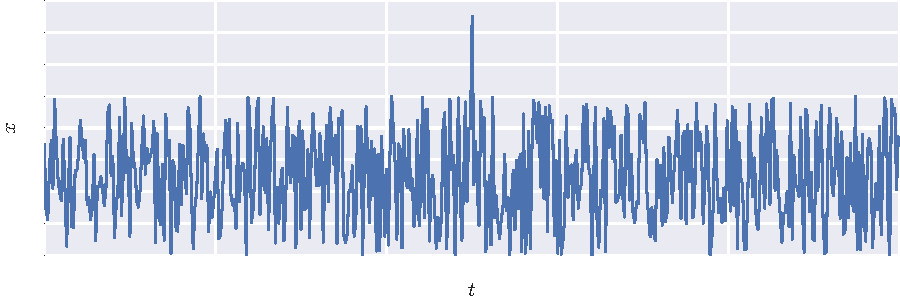
\includegraphics{figs/trivial.pdf}
  \caption{Simple Point Anomaly}
\end{figure}


\textbf{Context:} Some anomalies are defined within a context. In Figure \ref{fig:contextanom}, the anomalous point's value is within the range of the overall time series. But if the cyclic nature of the series were removed, the anomaly is readily detected (`converted' to a simple point anomaly).

\begin{figure}[H]
  \centering
  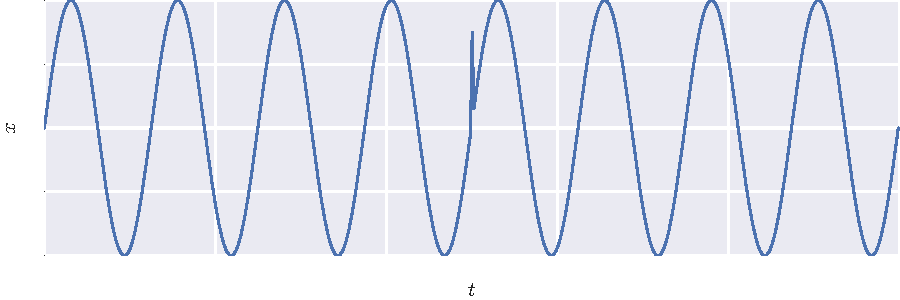
\includegraphics{figs/context.pdf}
  \caption{Anomaly in a Periodic Context}
  \label{fig:contextanom}
\end{figure}


\subsection{Discord}

Anomalies over subsequences are called discords \cite{Cheboli2010}. In Figure \ref{fig:perdiscordanom}, about two cycles in a periodic time series are unlike the other cycles. The repeated units do not have to be periodic as in Figure \ref{fig:aperdiscordanom}. 

\begin{figure}[H]
  \centering
  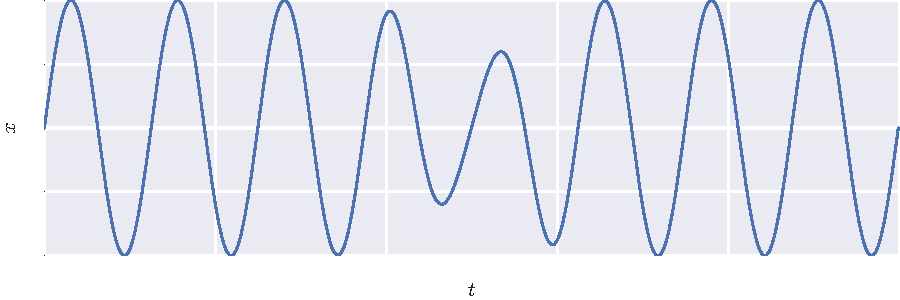
\includegraphics{figs/discord_per.pdf}
  \caption{Discord Anomaly in a Periodic Time Series}
  \label{fig:perdiscordanom}
\end{figure}

\begin{figure}[H]
  \centering
  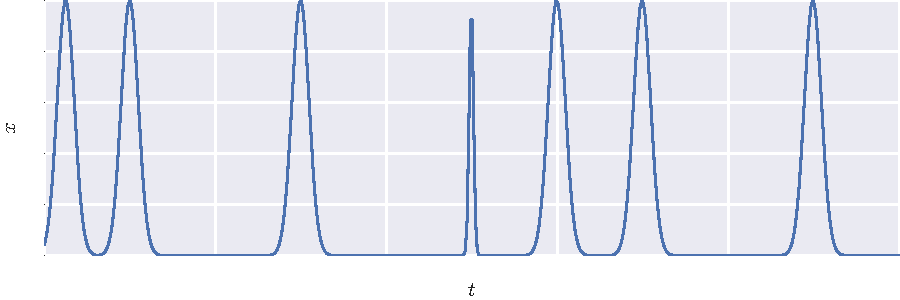
\includegraphics{figs/discord_aper.pdf}
  \caption{Discord Anomaly in an Aperiodic Time Series}
  \label{fig:aperdiscordanom}
\end{figure}

\subsection{Multivariate}

Multivariate time series add another element of complication for detecting anomalies in them and are not a focus of the thesis. \cite{Cheboli2010} classifies multivariate time series according to a combination of periodicity and synchronicity: Variables in a time series can be synchronous and periodic, syncronous and aperiodic, asynchronous and periodic, asyncronous and aperiodic. Therefore, any deviation from these properties are anomalies.

%%% Local Variables:
%%% mode: latex
%%% TeX-master: "thesis"
%%% End:

